%
% File ccl2024-zh.tex
%
%%
%% Based on the original version of COLING-2018 file (coling2018.tex), with changes made by Yue Zhang.
%%

\documentclass[11pt]{article}
\usepackage[utf8]{inputenc}
\usepackage[hyperref]{ccl2024-zh}
\usepackage{url}

%\usepackage{algorithm}
%\usepackage{algorithmicx}
%\usepackage{algpseudocode}
\usepackage[ruled,linesnumbered]{algorithm2e}

\usepackage{latexsym}
\usepackage{CJKutf8}

\usepackage{indentfirst}
\usepackage{fancyhdr}
\usepackage{graphicx}
\usepackage{tabularx}

\pagestyle{fancy}
\fancyhf{}
\lhead{\begin{CJK*}{UTF8}{gbsn}计算语言学\end{CJK*}}
\renewcommand{\headrulewidth}{0pt}

% \setlength\titlebox{5cm}

% You can expand the titlebox if you need extra space
% to show all the authors. Please do not make the titlebox
% smaller than 5cm (the original size); we will check this
% in the camera-ready version and ask you to change it back.



\title{面向CQL的语料库检索引擎的高效实现}
\englishtitle{Efficient implementation of a CQL-oriented corpus retrieval engine}

\date{}


\begin{document}
\begin{CJK*}{UTF8}{gbsn}
\setlength{\parindent}{2em}

% Make Chinese title and abstract
\maketitle
\begin{abstract}
  
本文提出了一种面向CQL的高效语料库检索引擎实现方法。首先,利用ANTLR工具对CQL语句进行语法分析,将得到的语法树转换为语料库检索式。其次,在构建语料数据库时,我们采用了优化的倒排索引表,实现了对非词表词语的快速检索。然后,在检索过程中,我们采取了两阶段策略:第一阶段忽略位置和距离约束,进行初步检索,并通过候选标记位方法迅速合并多个检索单元的候选列表;第二阶段则对候选列表应用约束条件进行二次匹配和过滤。最终,生成精确的候选语料列表。实验证明,该检索引擎在《人民日报》图文数据库上展现了高效且准确的性能,为语料库检索领域提供了新的解决方案和工程实践经验。

  \keywords{语料库查询语言 \and 语料库检索 \and 倒排索引}
\end{abstract}

% Make English title and abstract
\makeenglishtitle
\begin{englishabstract}
	
This paper proposes an efficient implementation method for a CQL-oriented corpus retrieval engine. Firstly, the ANTLR tool is utilized to perform syntactic analysis on CQL statements, converting the resulting syntax tree into a corpus retrieval expression. Secondly, when constructing the corpus database, we adopt an optimized inverted index table to enable rapid retrieval of non-lexical words. Then, during the retrieval process, we adopt a two-stage strategy: in the first stage, positional and distance constraints are ignored to perform preliminary retrieval, and the candidate lists of multiple retrieval units are quickly merged using the candidate marking method; in the second stage, constraint conditions are applied to the candidate lists for secondary matching and filtering. Finally, an accurate candidate corpus list is generated. Experiments demonstrate that this retrieval engine exhibits efficient and accurate performance on the People's Daily graphic database, providing a new solution and engineering practical experience for the field of corpus retrieval.

  
  \englishkeywords{corpus query language \and corpus retrieval \and  inverted index}
\end{englishabstract}


\section{引言}
\label{intro}

随着计算语言学领域的深入发展,语料库作为自然语言处理研究的基础资源,其重要性日益凸显。语料库检索引擎作为从语料库中获取信息的核心工具,其性能和效率直接影响到研究者的工作效率和成果质量。因此,构建一个高效、灵活的语料库检索引擎对于推动计算语言学研究具有重要意义。

目前,尽管已有一些语料库检索系统,例如:北京大学CCL现代汉语语料库、北京语言大学BCC语料库等中文语料库,拥有庞大的语料资源,提供了丰富的功能,但它们的检索表达式却互不兼容。这意味着用户在使用这些语料库时,需要分别学习和掌握各自的检索语法和规则。检索表达式的非通用性是一个突出问题,语料库检索的复杂性和多样性主要体现在其检索表达式的非标准化上。不同的语料库系统通常采用不同的检索语法,这导致了用户在使用不同系统时需要学习和适应不同的检索方式,增加了使用难度和成本。


%CQL作为一种通用的语料库查询语言,旨在提供一种统一的、易于学习和使用的检索语法,以简化用户在不同语料库系统之间的切换过程。通过实现一个高效的CQL检索引擎,我们可以为用户提供更加便捷、高效的语料库检索体验。

在本研究中,我们将重点探讨语料库检索引擎的实现,探讨如何使用更为通用的语料库检索语言进行语料库查询,以及如何建立语料数据库,优化索引结构的改进检索算法等。我们希望通过这些努力,为用户提供一个更加快速、准确、灵活的语料库检索工具,从而推动计算语言学研究的进一步发展。
%
%在计算语言学的研究领域中,语料库检索工具扮演着至关重要的角色。对于自然语言工作者而言,如何高效、准确地从庞大的语料库中检索到所需信息,是他们日常工作中必须面对的挑战。然而,目前语料库检索表达式的非通用性成为了制约其广泛应用的一大瓶颈。
%
%例如,
%
%CQL(Corpus Query Language)作为一种语法简单、易于掌握的语料库检索语言,得到了广泛的应用。然而,目前支持CQL的中文语料库还相对较少,这使得CQL的应用受到了一定程度的限制。
%
%
%设计一款能够支持CQL语言的语料库检索引擎,对于减轻用户学习负担、提高检索效率和质量具有重要意义。

%
% The following footnote without marker is needed for the camera-ready
% version of the paper.
% Comment out the instructions (first text) and uncomment the 8 lines
% under "final paper".
%
\cclfootnote{
    %
    % for review submission
    %
    \hspace{-0.65cm}  % space normally used by the marker
    % 最终版论文请将许可声明放在此处。请参阅说明中的~\ref{licence}部分来准备论文。
    \textcopyright 2024 中国计算语言学大会

    \noindent 根据《Creative Commons Attribution 4.0 International License》许可出版
}

\section{背景}
\label{backgound}

\subsection{CQL语言}

随着信息技术的飞速发展,语料库作为语言学研究的重要工具,其查询语言也经历了不断的演变与完善。其中,语料库查询语言(Corpus Query Language,简称CQL)作为从CQP(Corpus Query Processor)发展而来的一系列语言,已经逐渐成为语料库检索领域的主流语言。CQLF(Corpus Query Lingua Franca)已经成为国际标准ISO 24631-1 \cite{banski-etal-2016-corpus},在国际范围内的广泛认可与应用。

目前,众多语料库检索工具均采用了CQL作为检索语言,如CQPweb\cite{hardie2012cqpweb}、Sketch Engine\cite{sketchengine1}、BlackLab\cite{blacklab}等。这些工具使用CQL为用户提供高效、便捷的语料库检索体验。具体来说,CQL语言包括以下关键元素:

(1)查询语句:检索单元是由基本检索式以及逻辑运算符构成的,用于指定检索的标签以及具体的检索值。其中检索标签是在语料库设计时预先定义的,例如:word、lemmon、pos等。检索值即具体的查询内容,可以是词语、词性等。此外,CQL还支持使用正则表达式进行词语的匹配。简单查询可以通过布尔运算符进行连接,组成复合查询。一条查询语句可以包含多个检索单元,在语料匹配时,检索系统会对检索内容从左到右进行检索单元的匹配,每个检索单元还可以通过\{m,n\}的形式指定其重复次数。

(2)检索约束,CQL可以使用within操作符,限定检索范围。这使得用户可以在特定的文本片段进行检索。CQL还支持限定标签的使用,这用户可以对检索单元赋予一个标签名,然后通过"::"后面的限定条件,指定标签之间的逻辑关系,实现检索单元之间的条件约束。

\begin{table}[h]
	\begin{center}
		\begin{tabular}{|c|c|c|c|}
			\hline \bf 分类 & \bf 子类 & \bf 示例 & \bf 说明 \\ \hline
			查询语句 & 无约束 & [] & 匹配任意词语 \\
			查询语句 & 简单查询 & [word="在"] & 包含"在"的语料 \\
			查询语句 & 复合查询 & [word="花" \& tag="v" ] & 包含"花"作为动词的语料 \\
			查询语句 & 多段查询 & [word='他'][word='在'] & “他”、“在”连续出现的语料 \\
			查询语句 & 重复单元 & [word='不但'][]\{0,5\}[word='而且'] & "不但"和"而且"间隔5字内的语料 \\
			约束条件 & 范围约束 & [word='可以']within \textless s \textgreater & 在同一句中包含“可以”的语料 \\
			约束条件 & 限定标签 & A:[] [] B:[]  :: A.word = B.word	 & 包含形式为“ABA”词语的语料 \\
			\hline
		\end{tabular}
	\end{center}
	\caption{\label{font-table} CQL语句示例}
\end{table}

\subsection{倒排索引}

倒排索引是一种记录关键词出现在文档中的方式,通过记录关键词出现在那些文档的方式,建立关键词到文档的索引关系,从而提高搜索效率和匹配度。

在语料库设计中,需要根据语料库系统采用的标签,建立这些标签和文档之间的倒排索引信息。

语料库检索可以看作是通过标签信息检索到包含这些标签的文档的过程。语料库中一些常用的标签包括:词语、词语原型、词性等信息,这些都可以作为关键字建立标签与文档之间的倒排索引。

倒排索引技术,作为一种高效的信息检索手段,在现代信息处理和搜索引擎中发挥着关键作用。它的核心思想是根据文档内容生成一个索引,这个索引以单词或短语等关键元素为索引项,将文档中出现这些元素的位置信息或文档标识与之关联。通过这种方式,当用户输入查询请求时,系统能够迅速定位到包含相关元素的文档,从而极大地提高了检索速度和准确性。

具体来说,倒排索引的构建过程通常包括分词、统计词频、建立索引表等步骤。分词是将文本拆分成单词或短语的过程,而统计词频则是为了确定每个词在文档中的重要性。随后,系统会根据这些信息建立一个索引表,其中包含了词语到文档位置的映射关系。

在检索过程中,用户输入的查询请求会被系统解析成关键词,然后系统会在倒排索引中查找这些关键词对应的文档位置信息。由于倒排索引已经预先建立了关键词与文档之间的关联,因此系统能够迅速找到相关的文档,返回给用户。

倒排索引技术的优点在于其高效性和灵活性。通过预先建立索引,系统能够在短时间内处理大量的查询请求,同时支持复杂的查询操作和个性化的排序方式。此外,倒排索引还可以方便地支持增量更新和扩展,以适应不断变化的文档集合和查询需求。

%然而,倒排索引技术也面临一些挑战和限制。倒排索引对于语义信息的处理相对较弱,难以处理一些复杂的查询需求,如语义相似度匹配等。

Lucene是由Apache软件基金会提供的一套用于全文检索开源库,在全文索引和搜寻领域广泛使用。 BlackLab就是在Lucene基础上开发的语料库检索引擎。


\section{我们的工作}

我们选择CQL语言作为语料库检索语言。采用C++语言开发了一款高效的语料库检索引擎,采用ANTLR工具进行CQL语言的解析,确保了语法解析的准确性和高效性。同时,我们利用倒排索引技术建立了语料数据库,并针对CQL检索的特点进行存储结构设计以及性能优化,有效提升了检索速度和准确性,语料库检索流程如图\ref{fig:liucheng}所示。

\begin{figure}[!h]
	\centering
	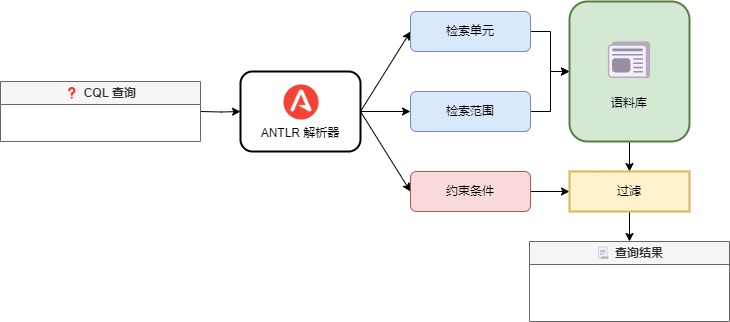
\includegraphics[width=0.7\textwidth]{image/liuchengtu.jpg}
	\caption{语料库检索流程图}
	\label{fig:liucheng}
\end{figure}


%我们还借助先进的大语言模型技术,实现了自然语言到CQL的转换功能。这一创新性的设计使得用户能够使用自然语言进行检索,无需掌握复杂的CQL语法,极大地降低了学习成本,提升了检索的便捷性。

\subsection{CQL语法解析}

CQL具有良好的人类可读性,但如果使用CQL实现语料库的检索,还需要将其转换为计算机可执行的结构化查询语句。
实现语法解析可以采用语法分析工具,ANTLR是一款强大的开源语法分析工具,使得开发一门新语言的工作转变为使用扩展巴斯科范式(Extended Backus–Naur Form,简称 EBNF)来描述语法。极大的简化了语言的解析工作。CQL符合EBNF定义,因此可以将CQL转换为EBNF语法文件。通过ANTLR工具,可以为CQL语法文件,生成相应的词法/语法分析器。
在\footnote[1]{https://github.com/exquery/corpusql-parser}提供的CQL语言描述文件的基础上,使用ANTLR工具生成了CQL的语法解析器。用户可以利用语法解析器将输入的CQL文本转换成语法树,语法解析器提供了Listener接口,可以通过该接口遍历语法树。
以“[word='把' \textbar word='被']”为例,生成的语法树结构如图\ref{fig:yufashu}所示:

\begin{figure}[!h]
	\centering
	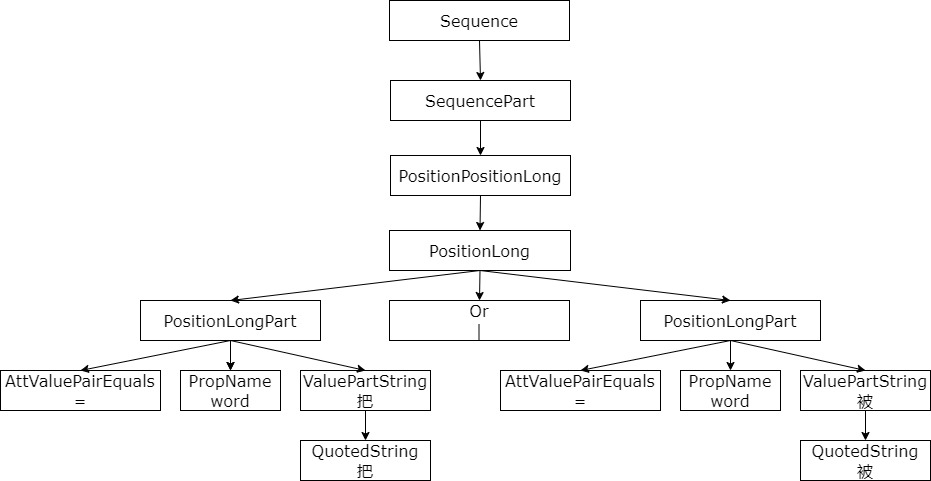
\includegraphics[width=0.7\textwidth]{image/yufashu.jpg}
	\caption{CQL语法树}
	\label{fig:yufashu}
\end{figure}

\subsection{倒排索引表设计}

检索和核心任务是完成检索词到文档的匹配,原始文本经过统一编码,段落分割、句子分割等预处理后,形成统一格式的语料数据。倒排索引工具,首先将传入的语料数据进行分段、分句操作,然后让每一句话通过分词工具进行分词以及标注词性,建立倒排索引表。

文档包含的信息是具有层次结构的,一篇文档,有很多属性信息包括:作者、文件名称、文件类型、文件大小、创建时间等信息,文件的内容还可以分为多个段落,每个段落由多个句子构成,在建立倒排索引时,根据语料库提供的范围约束条件,建立文档、段落、句子三级倒排索引结构。

用户输入的检索词不一定与语料库存储的词语一致,设计的倒排索引结构需要支持用户在文档中任意位置查询。比如在语料库中包含“北京市长”,被切分为“北京”、“市长”两个词语,但如果用户使用“北京市”检索时,仍然希望能够匹配到这份语料。因此倒排索引除了能够通过词语找到对应语料之外,还需要支持范围检索能力,能够根据用户的输入,找到与该输入匹配的语料的能力。

建立词语倒排索引分为四个步骤,第一步将语料库中文档ID化,即文档进行分词与词性标注,将文档内容转换为词语ID序列。第二步将ID化后的文档,依次遍历每一个词语ID,并以这个词语ID作为子句起点,加入排序列表,由于这个过程会产生大量的子句,因此在排序的时候按照子句句首词语进行分组排序。第三步,排序后获得了文档范围内所有词语的排序位置,生成词语排序位置索引表,这个表的数据可以看作是一个有序子句列表,可以直接用来检索匹配。第四步,为了优化检索速度,使用有序子句列表生成词语匹配范围表,词语匹配范围表直接可以通过词语ID返回词语在有序字句表中匹配的起始位置和结束位置。

\begin{figure}[!h]
	\centering
	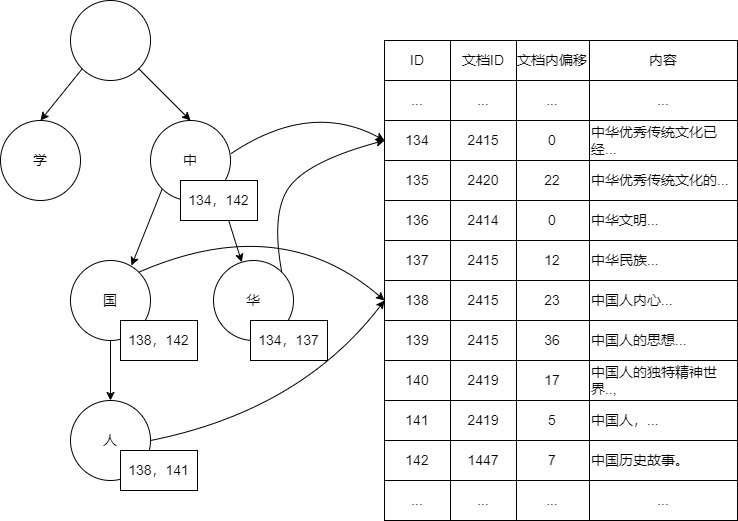
\includegraphics[width=0.8\textwidth]{image/daopaibiao.jpg}
	\caption{倒排索引表}
	\label{fig:daopaibiao}
\end{figure}

\subsection{语料库检索表达式}

在语料库查询时,需要将CQL转换为可执行的语料库检索表达式,该表达式包含三项内容:检索单元、约束条件、检索范围。检索单元是具体可执行的检索表达式,对应着CQL中的查询语句。约束条件是由查询语句中的无约束项以及限定标签转换出来的检索单元之间的约束条件。检索范围是CQL中的范围约束指定的检索范围约束条件。

\begin{figure}[h]
	\centering
	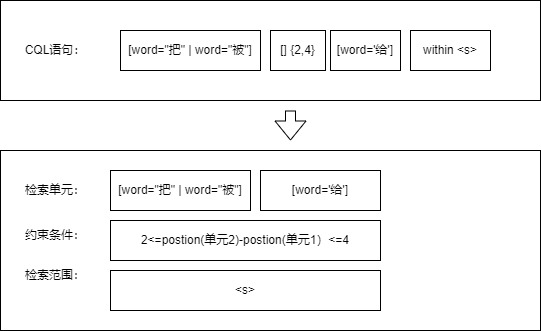
\includegraphics[width=0.5\textwidth]{image/jiansuoshi.jpg}
	\caption{语料库查询}
	\label{fig:jisnsuoshi}
\end{figure}

通过遍历CQL语法树,找到对应的节点,将节点元素转换为语料库查询表达式的元素,就可以调用语料库检索方法进行具体的语料查询了。

\subsection{二阶段候选查询}

语料库检索除了要对检索单元进行匹配外,还需要检查每个检索单元在语料中的位置是否满足位置和距离的约束,当存在多段检索单元时,如果能先过滤出满足检索单元匹配条件的句子之后,在进行约束条件的过滤和匹配,能够有效的提高检索效率。因此本文采用两阶段检索策略,第一阶段检索单元的匹配,搜索语料库执行检索单元的检索表达式,忽略检索单元的位置和距离约束,找到所有可能的匹配语料。第二阶段对上一阶段检索出来的语料进行位置和距离约束匹配,筛选出满足约束的语料作为候选。

第一阶段,检索单元匹配,首先根据检索范围选择相应的索引表,然后一次遍历执行每个检索单元中的检索表达式,如果检索单元是不包含逻辑运算的简单检索式可以在直接对应语料库的一次查询动作,根据标记类型,查找对应的倒排索引表,返回匹配的语料。包含逻辑运算的复合检索式,经过语法解析后,生成由简单检索式和逻辑运算符组成的检索树,通过遍历检索树并对每个简单检索式的检索结果按照逻辑运算符进行逻辑运算,即可返回复合检索式的检索结果。

合并不同检索单元,以及包含逻辑运算的检索单元内部的简单检索式的检索结果,是一个耗时操作,传统的倒排索引表存储的是排序好的文档ID列表,通过跳表操作实现两个列表的快速合并,但在我们设计的检索方法中,词语并不是固定的索引单位,并且词语对应的文档ID也不是有序的,无法采用合并有序列表的方式合并两个简单查询的结果。因此在我们的检索方法中,构建了一个与文档数量相同的一维bit数组,每一位标记着对应的文档是否匹配,合并两个检索表达式的之后,只需要执行检索式的逻辑运算,就可以快速完成合并操作。 
具体流程如算法~\ref{alg:getmatchdocflags}所示。

\begin{algorithm}[H]
	\caption{Get the query matching document ID flags}
	\label{alg:getmatchdocflags}
	\SetKwInput{KwInput}{$querys = \left\{ q_1, q_2, \ldots, q_n \right\}$}
	\SetKwInput{KwOutput}{$document\ id\ list$}
	\DontPrintSemicolon
	
	\KwInput{Input}
	\KwOutput{Output}
		
	% Set Function Names
	\SetKwFunction{FSum}{GetMatchDocFlags}
	
	% Write Function with word ``Def''
	\SetKwProg{Fn}{Def}{:}{}
	\Fn{\FSum{$query$}}{
		op = query.op\;
		\uIf {op = 'AND'} {
			flags1 $\leftarrow$ GetMatchDocFlags(query.first)\;
			flags2 $\leftarrow$ GetMatchDocFlags(query.second)\;
			flags $\leftarrow$ flag1 \& flags2\;
		}\uElseIf {op = 'OR'} {
			flags1 $\leftarrow$ GetMatchDocFlags(query.first)\;
			flags2 $\leftarrow$ GetMatchDocFlags(query.second)\;
			flags $\leftarrow$ flag1 \textbar \ flags2\;
		} \uElse {
			flags $\leftarrow$ SearchCorpus(query.data)\;
		}
		
		\KwRet flags\;
	}
	\;
flags $\leftarrow$ DefaultMatchFlags()\;
\ForEach{$q_i \in querys$}{
	flags $\leftarrow$ flags \& GetMatchDocFlags($q_i$)
}
	
	\KwRet flags\;
\end{algorithm}

第二阶段,位置距离约束,上一阶段返回的匹配文档,会根据检索语句中的约束条件类型反馈不同的数据,比如约束条件中由词性约束,则在返回的数据中就会包含词性信息。在执行约束条件时,从文档开始位置,一次检查检索单元的匹配位置是否复合约束条件要求。由于每个文档可能有多个位置与检索单元匹配,因此通过动态规划算法,从起始检索单元依次检查其中的匹配位置是否复合匹过滤条件要求,直到所有检索单元全部满足要求,将这一项加入到候选列表中。


%\subsection{自然语言查询}

%在本文中,我们参考了《从文本到 CQL:连接自然语言和语料库搜索引擎》这篇论文,利用大语言模型实现了自然语言到语料库检索语言(CQL)的转换,从而实现了使用自然语言进行语料库检索的目标。大语言模型具有强大的语言理解和生成能力,能够准确捕捉用户输入的语义信息,并将其转化为符合CQL规范的查询语句。通过这种方法,用户可以更加直观地表达自己的检索需求,无需了解复杂的CQL语法规则,提高了检索的便捷性和效率。实验结果表明,我们的大语言模型在转换自然语言到CQL方面取得了显著的效果,为语料库检索领域带来了新的突破。

\section{实验}

\subsection{数据集}

实验采用的数据集为《人民日报》图文数据库2014年-2015年的文本语料。在对数据进行分词以及词性标注后,通过本文创建的语料库搜索引擎,建立倒排索引表,生成语料数据库。然后编写典型的COL检索表达式,与CCL做对比测试。

\subsection{检索式对比}

CCL语料库检索式设计十分完善。然而,对于初学者而言,其学习成本相对较高。具体而言,CCL查询表达式中定义了多达13个特殊符号,其检索式由基本项、简单项、复杂项、过滤项、子句等多个部分组成,这就要求使用者必须掌握这些基础知识才能有效地编写检索表达式。

相比之下,CQL语言在语法上显得更为简洁直观。通过使用CQL表达式,用户能够更快速地掌握语料库的使用方法,无需投入过多的时间和精力去学习和记忆复杂的符号和规则。通过对比一些常用的检索式写法,我们可以清晰地看到CQL的简洁性。相较于CCL中使用的特殊符号和复杂的结构,CQL提供了一种更为直接和自然的方式来表达检索需求,从而提高了检索的效率和用户体验。

\begin{table}[h]
	\begin{center}
		\begin{tabular}{|c|c|c|}
			\hline \bf CCL检索式 & \bf CQL检索式 \\ \hline
			计算机硬件 & [word='计算机硬件'] \\
			把 \textbar 被 & [word='把'  word='给'] \\
			被+1把\$6给 & [word='被'][]\{1\}[word='把']\{0,6\}[word='给'] \\
			与其\$[2-4]不如 & [word = '与其'][]\{2,4\}[word = '不如'] \\
			
			\hline
		\end{tabular}
	\end{center}
	\caption{\label{font-table} CQL与CCL检索式对比}
\end{table}

通过对比可以看到,CCL检索式和CQL检索式能够实现的功能基本相同,但CQL检索式的形式和规则比较简单,采用统一的约束符号,更容易被掌握。

CCL的表达式,更为简洁,例如:查找同时含有“能力”和“大”的句子,且“能力”和“大”之间的间隔在3个字之内,二者的先后次序不受限制。使用CCL检索式编写:“能力\#3大” 能够实现这个功能,用CQL编写表达式为,A:[ word='能力' \textbar word='大'][]\{3,3\}B:[word='能力' \textbar word='大']::A!=B,较CCL繁琐很多。

\subsection{检索速度实验}

人工构造了10条检索式,选择《人民日报》2014-2015年数据进行检索速度对比试验,每个查询执行10次,取响应时间的平均值(单位:毫秒)。

\begin{table}[h]
	\begin{center}
		\begin{tabular}{|c|c|c|c|c|c|}
			\hline \bf CCL检索式 & \bf 数量 & \bf 时长& \bf CQL检索式 & \bf 数量 & \bf 时长 \\ \hline
			克服一切困难 & 10 & 10.0 & [word='克服一切困难'] & 8 & 3.6 \\
			好的\$10不好的 &15 & 52.0 & [word='的'][]\{0,10\}[word='的'] & 11 & 12.4 \\
			文化\$2交流 & 2138 & 24.0 & [word = '文化'][]\{0,2\}[word = '交流'] & 1921 & 9.5 \\
			把+1给 & 55 & 11.0 & [word='把'][]\{1,1\}[word='给'] & 24 & 8.7 \\
			与其\$[2-4]不如 & 38 & 21.0 & [word = '与其'][word = '不如'] & 34 & 4.9 \\
			(把 \textbar 被)\$[2-4]给 & 1010 & 19.0 & [word='把'  \textbar word='被'][]\{2,4\}[word='给'] & 1004 & 43.4 \\
			爱(X,1-3)不(X) & 13 & 10.0 & [word = '爱'][pos='v'][word = '不'][pos='v'] & 12 & 8.3 \\
			宁可\$10也 & 140 & 10.0 & [word = '宁可'][]\{\}[word = '也'] & 137 & 6.4 \\
			澡\$4洗 & 24 & 10.0 & [word = '澡'][ word = '洗'] & 19 & 5.3 \\
			一边+3一边 & 131 & 15.0 & [word = '一边'][]\{3,3\}[word = '一边'] & 131 & 7.4 \\
			\hline
		\end{tabular}
	\end{center}
	\caption{\label{font-table} 与CCL查询速度对比}
\end{table}

检索到的文档数量上存在一定的差异,原因是数据预处理造成了文本内容差异,以及使用的分词工具不同,造成的检索匹配单元不一致造成的。通过数据对比,可以看到设计的检索引擎的检索速度在多数情况下优于CCL,平均检索速度快40\%(110.9/182) 。

\section{结论}

本文对语料库检索进行深入探索,采用CQL作为语言库检索语言,通过ANTLR工具将CQL语言解析问语法树,设计和构建了C++版本的语料库检索引擎,采用二阶段检索策略,以及候选标记位过滤方案,提升语料库的检索速度,实现表明本文设计的检索引擎高效准确。
\cite{li2023can}
综上所述,本文实现的面向CQL语言语料库检索引擎,为构建语料库检索提供了解决方案以及工程实践经验。


% include your own bib file like this:
\bibliographystyle{ccl}
%\bibliography{ccl2022-zh}
\bibliography{custom}

\end{CJK*}
\end{document}

